%% !TEX root = ../ThesisManuscript_SJ.tex
%%
%%
%%	INTRODUCTION
%%_______________________________________________
\chapter{General introduction} 
\label{Introduction} 
\markboth{GENERAL INTRODUCTION}{}

\addtocontents{lof}{\protect\contentsline{chapter}{\protect\numberline{}Chapter \thechapter \medskip}{}{}}
\addtocontents{lot}{\protect\contentsline{chapter}{\protect\numberline{}Chapter \thechapter \medskip}{}{}}

\section{Prevention interventions aiming to the elimination of infectious diseases}
\label{Intro:Prevention}

The prevention of infectious diseases has greatly improved, not only as a result of the development of safe, highly-effective preventive %and therapeutical 
methods, but also thanks to regional and global public health programs aiming at infectious diseases' elimination. Immunization alone can now prevent more than 20 life-threatening diseases \cite[]{WHO_IA2030}. Mass immunization programs achieved the eradication of smallpox in 1980\footnote{During the pre-vaccination era, the mortality rate due to smallpox infection were about 30\% \cite[]{CDC_Smallpox2001}.} \cite[]{CDC_Smallpox2001}. The number of cases of poliomyelitis (commonly known as polio) has decreased from an estimated 350~000 cases in 1988, to 33 reported cases in 2018 \cite[]{WHO_Factsheet_Polio}. %The incidence of meningococcal meningitis has decreased by 58\% in a relatively short period of time \cite[]{WHO_Factsheet_Meningitis}. 
Between 2000 and 2018, vaccination against measles prevented an estimated 23 million deaths \cite[]{WHO_Factsheet_Measles}. During the same period, the number of new HIV infections fell by 39\%, thanks to preventive interventions \cite[]{WHO_Factsheet_HIV}. Preventive interventions have decreased the overall number of new infections worldwide \cite[]{CDC_10achievements} and placed some communicable diseases, such as measles and poliomyelitis, in the path towards elimination \cite[]{CDC_10achievements}. 
 
During the last decade, the World Health Organization (WHO) developed the Global Vaccine Action Plan (GVAP) 2011--2020, aiming to ensure individuals to live free from vaccine-preventable diseases \cite[]{GVAP_Review2020}. As a result, vaccine coverage among children and vaccine development have shown a remarkable progress, but many other objectives remained unmet \cite[]{GVAP_Review2020}. Disease-specific programs were also developed to fight infectious diseases' epidemics; for instance, the Global Measles and Rubella Strategic Plan 2012--2020 \cite[]{WHO_MR2012} and the Fast Track to end AIDS epidemic \cite[]{UNAIDS_EndAIDS2011}. 

%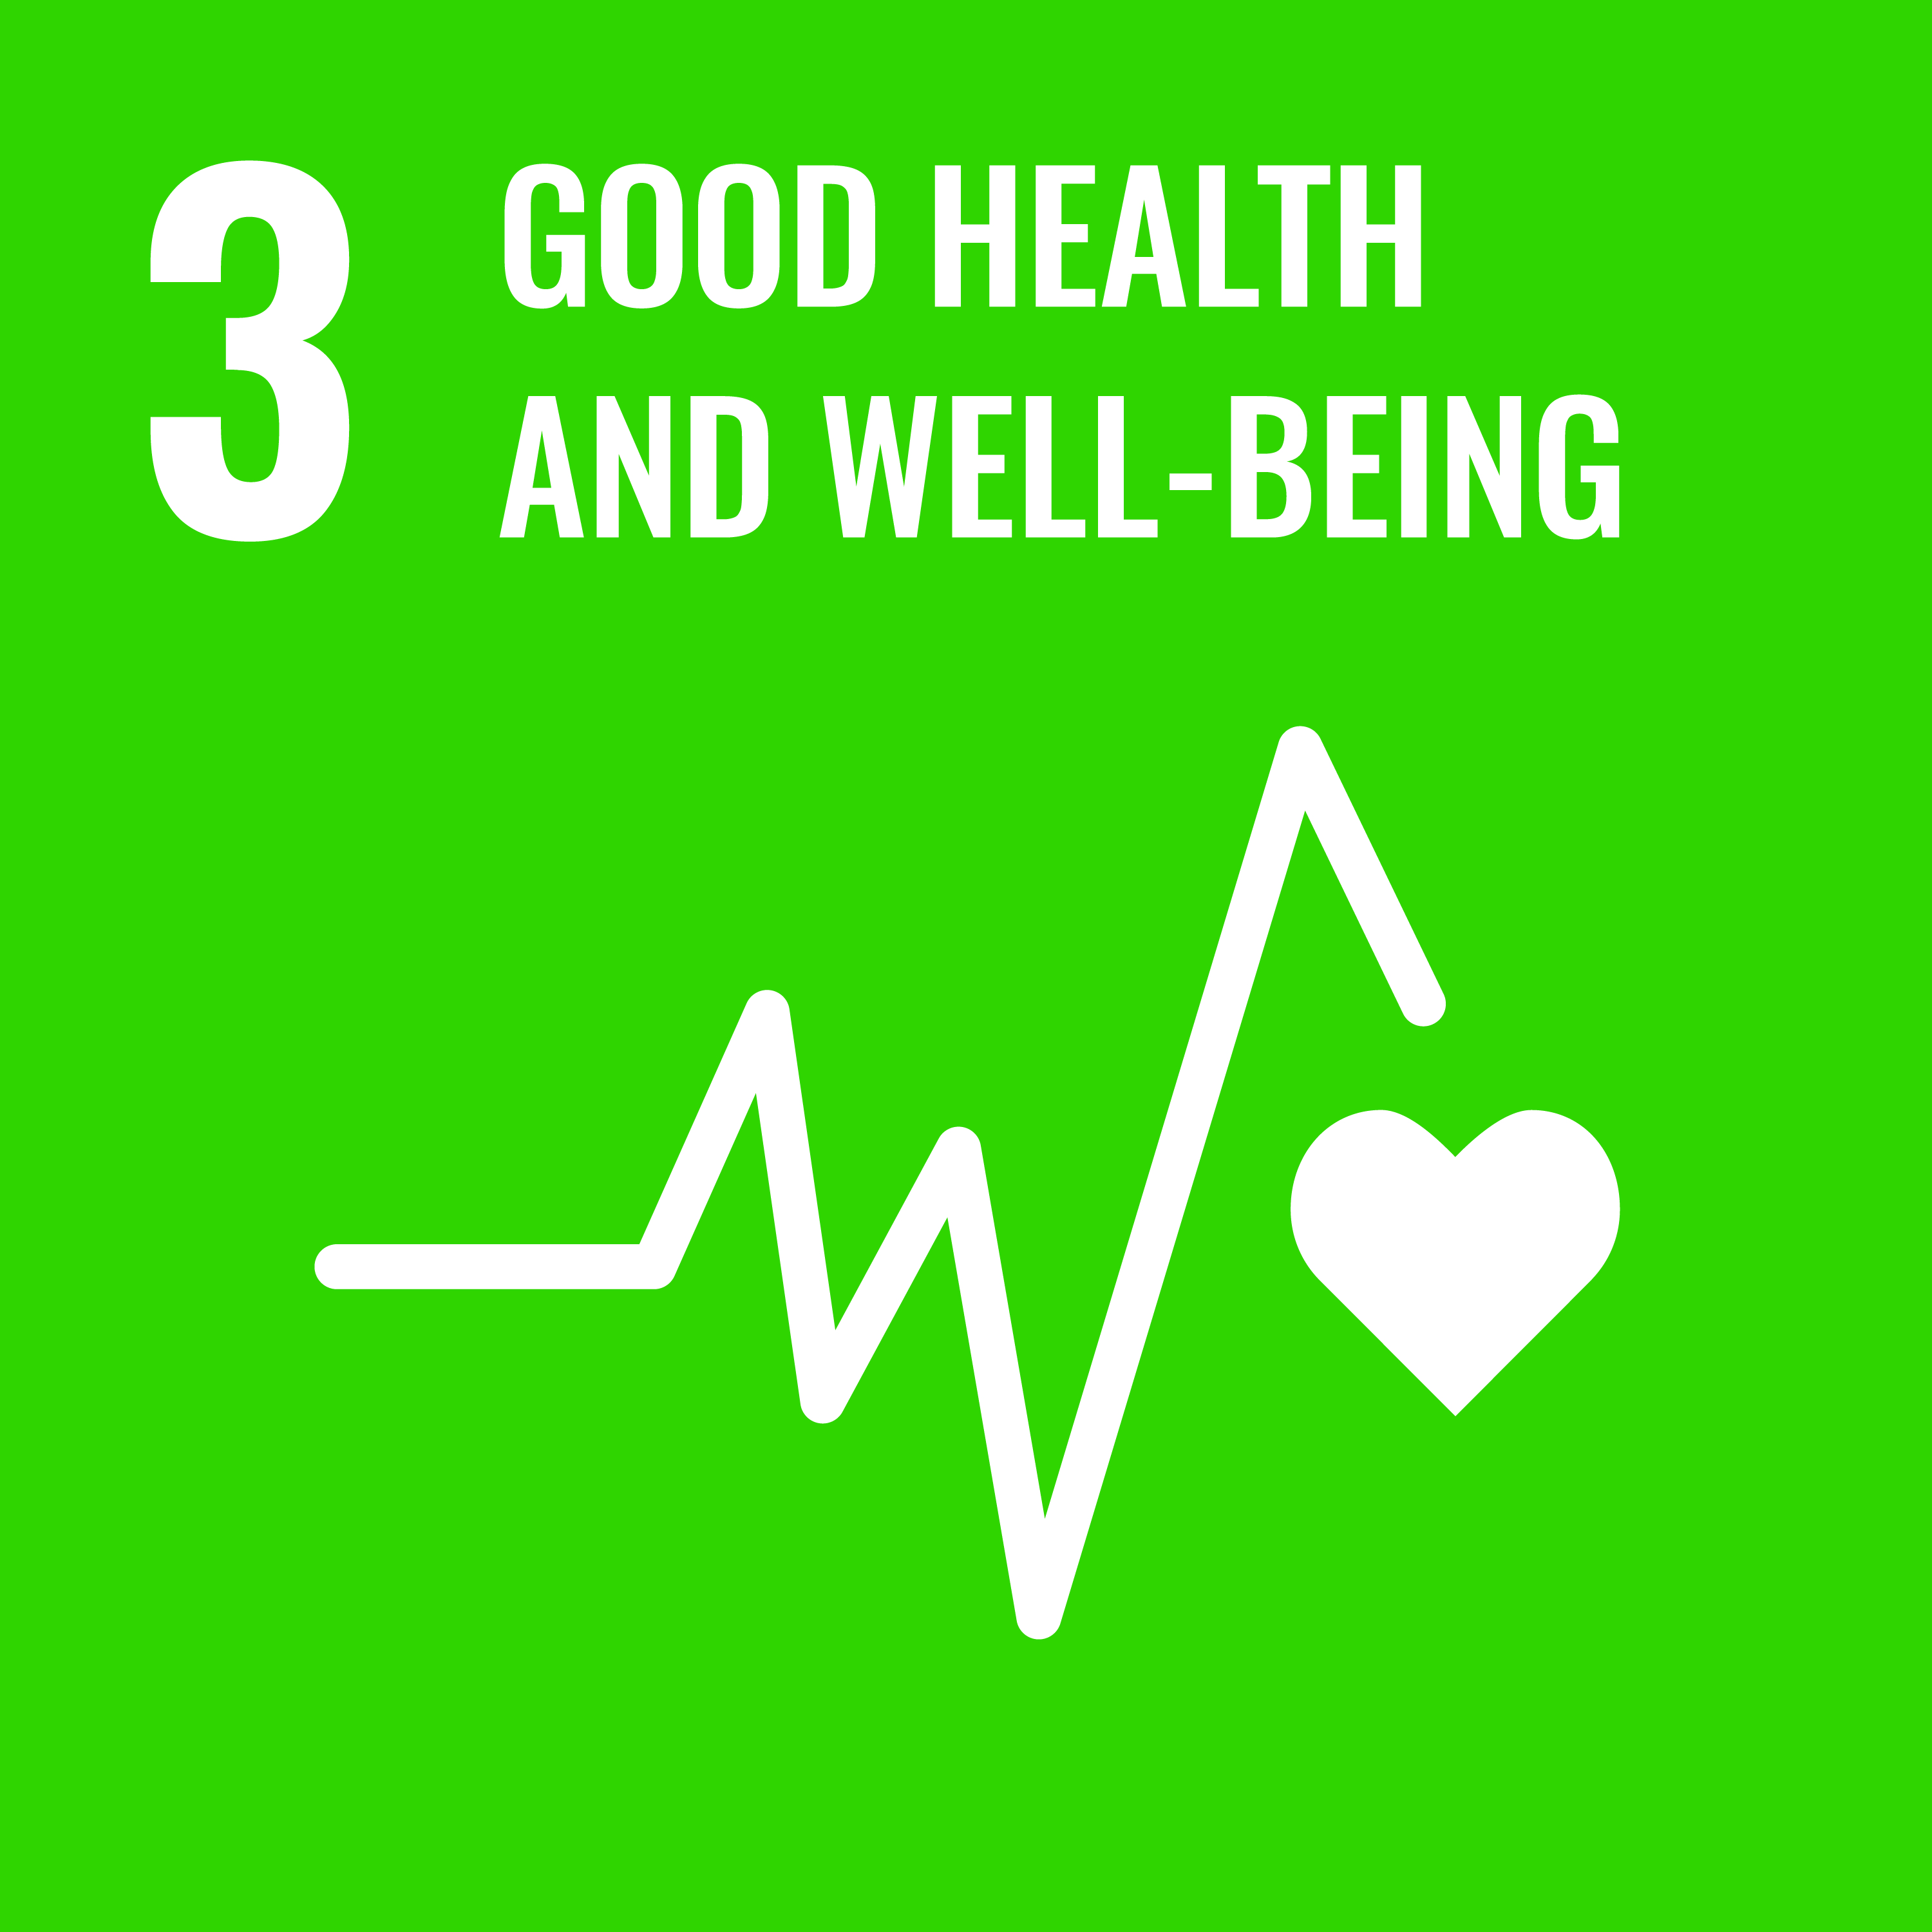
\includegraphics[width=2cm]{Figures/Intro/Goal3_SDG} 

Nowadays, disease-prevention interventions are included in the WHO's 17 Sustainable Development Goals; specifically, in the 3rd goal: ``To ensure healthy lives and promote well-being for all at all ages'' \cite[]{SDG_Goal3}. The objectives concerning communicable diseases include to end, by 2030, the epidemics of AIDS, tuberculosis, malaria and neglected tropical diseases, as well as to end preventable deaths of newborns and children under 5 years of age \cite[]{SDG_Goal3}. As a result, the currently ongoing Immunization Agenda 2030, the successor of the GVAP 2011--2020, places immunization in the core of national strategies for primary health care and universal health coverage~ \cite[]{WHO_IA2030}. In parallel, a global program to end sexually transmitted diseases by 2030 is ongoing, aiming, for instance, at the elimination of cervical cancer through vaccination interventions against human papillomavirus \cite[]{WHO_STIs}. The Fast Track initiative to end the AIDS
%\footnote{Disease caused by the HIV virus, which targets the immune system, reducing the defense against other infections \cite[]{WHO_Factsheet_HIV}.} 
epidemic is still ongoing, setting more ambitious and inclusive targets \cite[]{UNAIDS_EndAIDS2030}. 


\subsection{Epidemic elimination}  \label{Intro:EpiElim}

Unlike infectious disease \emph{eradication}, which is defined as the complete termination of disease transmission or the total elimination of the infectious agent \cite[]{Porta2014}, there is no consensus for the definition of disease and epidemic \emph{elimination}. Global (respectively, regional) epidemic elimination often refers to the end of an epidemic as a public health concern, through a high or a complete reduction of the infectious disease transmission worldwide (respectively, in the region), during a period of active surveillance \cite[]{Porta2014,Nishiura2016}. Global and regional programs aiming at disease elimination set specific targets to be met in a certain amount of time and thus, declaring disease elimination may depend on the specific infectious disease and its context. See table~\ref{table:InfDisElim} for some disease-specific targets currently included in WHO programs aiming at regional and/or global elimination.

The classical approach of the WHO to declare the end of an epidemic is to observe no new cases after a significant period of time after the last reported case \cite[]{Nishiura2016}; for instance, twice as long as the empirical maximum of the incubation period. Other, rather heuristic ways to determine the end of an epidemic have also been used: the end of a Middle East respiratory syndrome (MERS) outbreak in South Korea was declared after the removal of movement restriction for the last quarantined case, which was almost a week before the date that would have be determined by the WHO criteria \cite[]{Nishiura2016}. 

However, the case-free period approach to determine disease elimination may depend highly on the sample size, be inappropriate for diseases with high proportions of asymptomatic cases \cite[]{Nishiura2016}, and depend greatly on prevention coverage \cite[]{Eichner1996}. Mathematical models can help overcome some of these difficulties. For instance, modeling studies have found that asymptomatic cases of poliomyelitis infection may still occur with a probability lower than 1\%, 5 years after having no symptomatic cases within a population of 200\,000 \cite[]{Eichner1996}. In addition, mathematical modeling may provide estimates for unobserved disease parameters, as well as identify the criteria to be met to end an epidemic; thus being useful to set public health targets for epidemic elimination.

\begin{landscape}
\captionsetup{width=1.3\textwidth}
\begin{table}[H]
	\centering
	\small
	\begin{tabular}{llll}
	\toprule
	\bf Infectious disease & \bf  Main targets & \bf Target year &\bf Ref.\\
	\toprule
AIDS				& $\bullet$ 95\% of infected people to know their HIV status & 2030 & \cite{UNAIDS_EndAIDS2030}\\
				& $\bullet$ 95\% of diagnosed people to be on treatment & &\\
				& $\bullet$ 95\% of people on treatment to have suppressed viral load & &\\ \midrule
	\bf Measles 	& $\bullet$ Absence of cases for at least 3 years & 2020\textsuperscript{a,b}  &  \cite[]{WHO_GVAP2018} \\
				& $\bullet$ High regional coverage of vaccination & &\\\midrule
	\bf Poliomyelitis & $\bullet$ Absence of cases for at least 3 years &&\cite[]{Eichner1996}\\
				& $\bullet$ No circulation of wild strains & &\\ \midrule
	\bf Rubella 	& $\bullet$ 95\% reduction in the regional number of cases & 2020\textsuperscript{b}  & \cite[]{WHO_GVAP2018}\\
				& $\bullet$ Absence of cases for at least 3 years  & &\\
				& $\bullet$ High regional coverage of vaccination & &\\ \midrule
%	\bf Viral hepatitis & Reduce new cases of chronic viral hepatitis B infections by 95\% & 2030 & \cite[]{UN_IA2030}\\
	\bf Yellow fever & $\bullet$ Reduction of the number of outbreaks to none & 2026 & \cite[]{WHO_IA2030}\\
	\bottomrule
\end{tabular}
	\caption[Targets of some recent, global WHO programs aiming to end infectious diseases epidemics]{%
	\textbf{Targets of some recent, global WHO programs aiming to end infectious diseases epidemics}\\
	{\rule{5.5cm}{0.5pt}\\
	\footnotesize
	\textsuperscript{a} The American region was certified as having eliminated measles in 2016, after high vaccination coverage efforts, but lost its certification in 2018, after observing several outbreaks. Measles is currently endemic in all regions \cite[]{GVAP_Review2020}.\\
	\textsuperscript{b} Unmet targets.}
	}
\label{table:InfDisElim}
\end{table}
\end{landscape}

%\subsubsection{The prevention of infectious diseases: a multi-disciplinary, multi-level challenge}
%
%\rev{The success of public health programs aiming to epidemic elimination relies on many ... at many different levels. From the development of effective preventive and therapeutic tools, to the logistics ensuring availability and facilitating access. International or regional epidemiological targets require joint research and collaboration at the same scale. At the same time, the program implementations' adaptation to the local infrastructure and socio-cultural contexts is essential. }
%
%Ressource allocation and research funding. Public health authorities deploy prevention programs, ensuring constant feedback from the public, gathering surveillance data and sharing it with the public. 
%
%Prevention program also on the public participation, and thus, depend on the individual acceptance and adoption of the interventions. Hence, the role of the media and communication departments becomes important too, for an informed decision-making needs clear, accurate, opportune information. 
%
%Here, we focus in the role of the individual-level decision-making, facing epidemic threat in a context where efficient preventive and therapeutic methods are available, from the epidemiological and mathematical modeling perspective.

\section{The prevention versus treatment dilemma}
\label{Intro:Dilemma}

``An ounce of prevention is worth a pound of cure'', goes the popular saying. Yet, the individuals' preference for prevention over treatment may not be guaranteed. Some studies have indeed found a preference for prevention \cite[]{Bosworth2010,Mortimer2008}, while others have found a preference for treatment \cite[]{Corso2002,Schwappach2002} or not a significant preference \cite[]{Ubel1998}. Preference has also been found to vary widely depending, for instance, on age and health state \cite[]{Luyten2015} or the perception of the urgency of adopting a preventive intervention \cite[]{Meertens2013}. Individuals' attitudes towards prevention may thus differ from the public health authorities' recommendations. Therefore, when facing the risk of an epidemic, in a context where efficient treatment is available, individuals who find themselves at risk of infection may engage in a \textit{prevention versus treatment dilemma}, and make the decision between adopting  or not prevention, while having the option for treatment in the case of infection. 

\textit{Voluntary prevention} is defined as the preventive methods adopted voluntarily by individuals to avoid infection, that is, by willingly following the recommendations of public health authorities' --- in contrast to mandatory prevention (i.e., required by law or community rules). The voluntary adoption of prevention mainly depends on the individuals' perception of its benefits and inconveniences versus those of treatment, as well as their perception on their own risk of infection, and of the consequences of being infected. Public health authorities and healthcare providers may play an essential role shaping these perceptions: by sharing information about epidemics and disease burden, as well as providing information on the available preventive and therapeutic tools, and increasing their availability and facilitating access.% \cite[]{Larson2016,Coleman2017}.

To evaluate the impact of voluntary prevention on the epidemic dynamics, in the context where efficient treatment exists, it is thus essential to account for individuals' resolution of the prevention versus treatment dilemma. Here, we focus on the role of decision-making by individuals facing epidemic threat in a context where efficient preventive and therapeutic methods are available, from the epidemiological and mathematical modeling perspective.

\section{Mathematical and behavioral epidemiology}
\label{Intro:BehavEpi} 

Mathematical modeling of infectious diseases was used to assist public health decision-making for the first time in 1760\footnote{The paper was first presented at the Royal Academy of Sciences in Paris in 1760 and then published in 1766 \cite[]{Bernoulli1766}.}, when Daniel Bernoulli (1700--1782) studied the smallpox epidemic and recommended universal variolation to alleviate smallpox-related mortality: ``...it has been noticed that, on the one hand, the more natural smallpox spreads, the more dangerous it is; and, on the other, that inoculation carried out at the height of an epidemic is not by any means as reliable as if it were done quite outside any epidemic'' \cite[]{Blower2004}. Bernoulli's recommendation was based on his estimation of the number of lives saved by universal inoculation against smallpox \cite[]{Blower2004}. The model proposed by Bernoulli consisted in analyzing surveillance data on the yearly number of individuals who had been infected, the number of deaths due to smallpox infection, etc. Then, he compared the number of smallpox deaths before and after the adoption of inoculation amid the population \cite[]{Blower2004,Dietz2002}. In his paper, Bernoulli also acknowledged that individuals could be interested in being inoculated because of the benefits it offered at the individual level (such as avoiding lethal infection), versus those offered at the population level (such as increasing the average life expectancy).

Since the 18th century, different kinds of mathematical models have been developed to describe epidemic dynamics \cite[]{Brauer2017}. Models can be useful to understand the transmission mechanisms behind surveillance data, to estimate the values of disease parameters that cannot be directly measured, to predict disease epidemiology and to select intervention designs aiming to control the epidemic and or the disease burden \cite[]{Valleron2000}. Mathematical epidemiology has thus become a powerful tool for public health decision-making and epidemic control \cite[]{Valleron2000}. 

Behavioral epidemiology is a relatively recent branch of mathematical epidemiology arising from the need to include, explicitly, the behavioral changes of individuals facing epidemics. Epidemic dynamics are coupled to behavioral dynamics, which are determined, for instance, by the individuals' attitudes towards preventive and therapeutic tools and/or compliance to public health policies. Behavioral epidemiology thus studies the interplay between human behavior and the course of an epidemic, by considering human behavior as a key component of both epidemic spread and the implementation of public health policies \cite[]{Bauch2013}. The scientific production in the field may be found in an overview of the early growth of behavioral epidemiology by \cite{Bauch2013} and an article review covering the period 2010--2015 by \cite{Verelst2016}. In addition, a review by \cite{Wang2016} focused in mathematical epidemiology of vaccination includes a large section on behavioral models, and a review by \cite{Wang2015} presents models of epidemic spread through contact networks accounting for changes in the individual behaviors.%, which was commented by \cite{Rosati2015}, to also consider the work on complex networks that fit the models to available data.

From the modeling perspective, the issue of voluntary prevention and its impact on epidemics has been addressed using hybrid models that combine mathematical models describing the disease transmission at the population level, with models describing the individual's adoption of preventive methods to avoid being infected \cite[]{Verelst2016}. The infectious disease transmission has been modeled using mostly deterministic compartimental models\footnote{As opposed to stochastic models (that can also be compartmental), which can be particularly useful to model disease transmission among small populations.}  and individual-based models (which allow to consider stochasticity and high heterogeneity between individuals). The adoption of prevention has been modeled, for instance, by a change in the individual's susceptibility to the infection (such as being immunized), a change in the model parameters (such as reducing disease transmissibility) or a change in the contact structure (such as reducing the number of contacts with other individuals, which is known as \textit{social distancing}); see \cite{Verelst2016}. Traditionally, hybrid models studying social distancing use the individual-based models for the disease transmission, while those studying vaccination use compartimental models \cite[]{Verelst2016}.

In behavioral epidemiology, individuals are assumed to translate the information about epidemic dynamics into behavioral changes; i.e., acknowledging their risk of infection and making informed decisions. The information about the epidemic has been previously modeled as epidemiological indicators ---assumed to be provided to individuals by public health authorities---, as well as subjective perceptions and/or rumors \cite[]{Verelst2016}. The interaction between the information about the epidemic and the change in behavior has been modeled, for instance, as a threshold that triggers the prevention adoption, as a dynamic parameter which affects and is affected by prevention adoption or as a transfer between compartments explicitly representing the awareness level of the individual \cite[]{Verelst2016}. Other models based in networked populations have used multiple layers to couple the epidemic-spreading network to a `virtual' information-spreading network \cite[]{Wang2016}. Some models have used the risk of infection perceived by individuals to explicitly address the prevention versus treatment dilemma (see~\secref{Intro:DecisionModel}). Only a few hybrid models have been calibrated using available data \cite[]{Verelst2016}.

							
\subsection{Modeling disease transmission using deterministic compartmental models}

Deterministic compartimental models have been widely used to model disease progression and transmission among large populations since 1900 \cite[]{Brauer2017}. These models can be expressed as a system of ordinary differential equations (ODE), whose state variables represent the number or proportion of individuals in each compartment, and whose parameters relate to the rates of transition from one compartment to another \cite[]{Hethcote2000}; for instance, from susceptible to infected, then to infectious or contagious, to recovered, susceptible again, or dead, and so on. The transition of individuals from being susceptible to being infected, is often modeled by the the rate of infection, also called \textit{force of infection}. The force of infection may be defined by a constant rate or by a function, depending explicitly on the disease transmission mechanisms, such as the contacts between uninfected and infectious individuals, and their probabilities to occur. 

Classical compartmental models are usually named by acronyms obtained from merging the initials of the compartment variables. For instance, a model considering only susceptible, infected and recovered individuals is called an $SIR$ model. The Bernoulli's paper mentioned in the previous section can be represented by an $SI$ model \cite[]{Dietz2002}. \hyperlink{fig:Intro_VSIR}{Figure~\ref*{fig:Intro_VSIR}} depicts a paradigm example of a compartmental model accounting for prevention adoption. Susceptible individuals ($S$) can get infected ($I$) and then recover ($R$), or die at any time. A compartment for the proportion of susceptible individuals who adopt prevention ($P$) is added to the model; the classical $SIR$ thus becomes an $PSIR$ model. An imperfect preventive method is modeled, for instance, by individuals getting infected despite using prevention and by waining protection (useful for modeling waning immunity in vaccination models) \footnote{On the contrary, in the case where perfect prevention is considered,  individuals using prevention are immune to the disease and thus directly removed from the population --- to the $R$ compartment.}. 

\begin{figure}[H]
	\centering	
	%% DRAFT
%	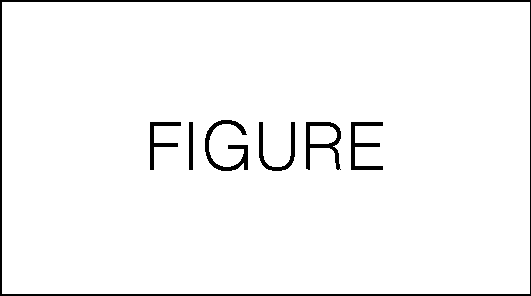
\includegraphics[width=0.6\textwidth]{DRAFT_FigsAndDocs/FIG}
	%%
	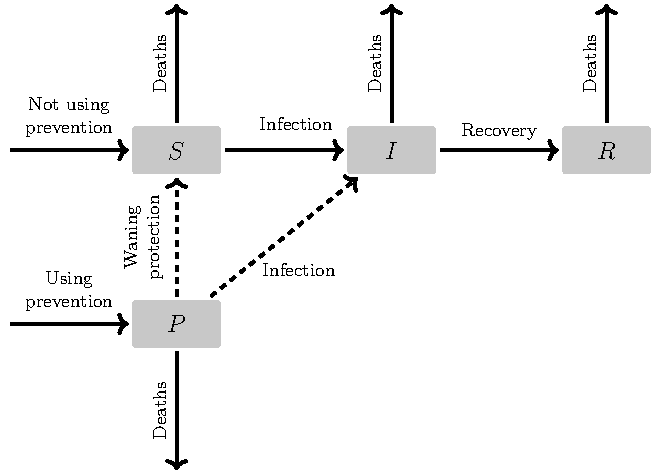
\includegraphics[width=0.6\textwidth]{Figures/Intro/TikZ_PSIR/PSIR_FlowDiagram}
	\caption[ Conceptual compartimental model with prevention]{%
		{\bf Conceptual compartimental model with prevention}\\
		\raggedright
		Flow diagram of a classical \textit{SIR}-type compartimental model accounting for prevention adoption. The model describes the transmission of an infectious agent  and disease progression, within a population by modeling individuals' transitions through different states, during their lifetime. Individuals may use prevention ($P$) against the infectious disease or not. Susceptible ($S$) individuals get infected ($I$) and then recover ($R$). An imperfect preventive method is modeled, for instance, by individuals getting infected despite using prevention, and/or by waning the protection offered by the preventive method with time (dashed arrows).}
	\label{fig:Intro_VSIR}
\end{figure}
 
More complex compartmental models can include population stratification by disease progression (e.g., acute infection, chronic or asymptomatic period), case resolutions (e.g., removal, recovery, death), demographics (e.g., age, sex), exposure to the disease (e.g., risk of infection, number of contacts), use of preventive and/or therapeutic tools, etc.; see \cite{Hethcote2000}. 


%\subsection{Using the basic and the effective reproduction numbers to determine the impact of preventive methods}
\subsection{The basic and the effective reproduction numbers}
\label{Intro:ReproductionNumbers}

The \textit{basic reproduction number}, noted $R_0$, is defined as the expected number of secondary cases produced by a single infectious individual, during the entire infectious period, in a fully susceptible population \cite[]{Anderson1991,Heesterbeek2002}. The \textit{effective reproduction number} ---also called the replacement number--- is defined as the expected number of secondary cases produced by an infectious individual, at a given time or in a given context; for instance, once the population is subject to interventions such as prevention and treatment \cite[]{Ridenhour2018,VanDenDriessche2008,VanDenDriessche2002,Hethcote2000}. % In other words, the effective reproduction number represents the number of secondary infections occurring at a time $t$, whereas the basic reproduction number represents a theoretical number of secondary cases occurring in the absence of previous infections and interventions, and thus, independent of time.

The basic and the effective reproduction numbers reflect epidemic severity, and thus are useful to study the impact of preventive methods on epidemic dynamics: a large basic reproduction number may be interpreted as a fast epidemic spread among the susceptible population exposed to the infectious disease; a decrease in the effective reproduction number reflects epidemic mitigation. 

The basic and the effective reproduction numbers can be estimated from mathematical models \cite[]{Ridenhour2018}. In particular, they can be computed from deterministic compartmental models, and thus be expressed as functions of the ODE system parameters \cite[]{Heffernan2005}. Notably, there exists a relation between the reproduction numbers and the behavior of the ODE system at the equilibrium \cite[]{VanDenDriessche2002,VanDenDriessche2008}. ODE systems defining classical compartimental models for disease transmission, similar to the model depicted in~\figref{fig:Intro_VSIR}, often have two equilibria: a disease-free state (DFS), where there are no new infections, and an endemic state (ES), where the epidemic persists \cite[]{Hethcote2000,VanDenDriessche2002}. A reproduction number is a threshold parameter for the ODE system equilibria: there is a transcritical bifurcation (that is, an exchange in the stability between the equilibria) for the ODE system when the reproduction number equals to 1. When the reproduction number is lower than 1, the ODE system reaches the DFS and thus the epidemic is eliminated in the long run; otherwise, the ODE system will reach the ES \cite[]{Hethcote2000,VanDenDriessche2002}. See~\figref{fig:Intro_Bifurcation} for a conceptual visualization of the transcritical bifurcation.

\begin{figure}[H]
	\centering	
	%% DRAFT
%	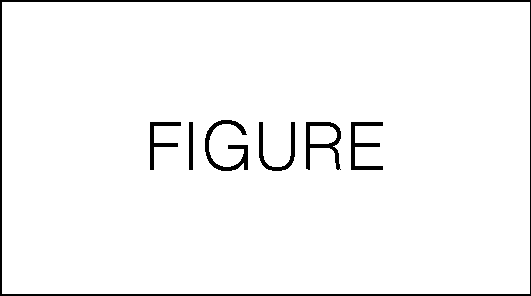
\includegraphics[width=0.7\textwidth]{DRAFT_FigsAndDocs/FIG}
	%%
	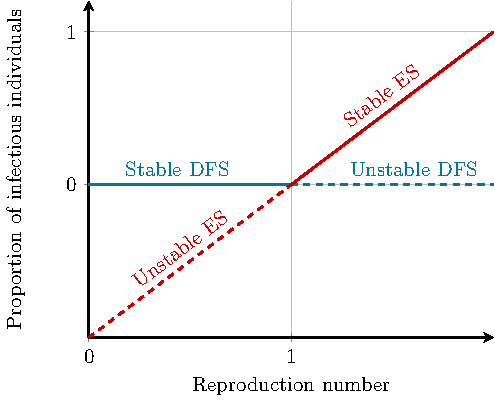
\includegraphics{Figures/Intro/TikZ_Bifurcation/TranscriticalBifurcation}
	\caption[ Conceptual diagram of a bifurcation in the ODE system]{%
		{\bf Conceptual diagram of a bifurcation in the ODE system}\\
		\raggedright
		Classical systems of ordinary differential equations (ODE) describing disease transmission usually have two equilibria: the disease-free state (DFS, depicted in blue), where there are no new infections, and the endemic state (ES, depicted in red), where the epidemic persists. A change in the stability of the equilibria occurs when the reproduction number equals to 1 (depicted by the transition from a solid to a dashed line). Note that negative populations (red, dashed line), while corresponding to the solutions of the ODE system, have no biological interpretation.}
	\label{fig:Intro_Bifurcation}
\end{figure}

\subsubsection{Using the reproduction numbers to determine the herd immunity threshold} 
\label{sec:Intro_HerdImmunity}

Prevention-induced \textit{herd} or \textit{community immunity} refers to the situation in which susceptible individuals are indirectly protected against infection, due to a sufficiently large prevention coverage (i.e., the proportion of the population adopting the preventive method against the pathogen) \cite[]{Porta2014}. As a result, disease transmission is greatly reduced and the population is said to be immune as a group; the epidemic is expected to be eliminated in the long run (i.e., the DFS is reached); see \cite{Fine2011}.

From the modeling perspective, the prevention coverage required for the community to reach herd immunity may be obtained by identifying the prevention coverage yielding an effective reproduction number\footnote{The effective reproduction number depends (implicitly or explicitly, depending on the modeling choices) on the preventive coverage.} lower than 1. The larger the basic reproduction number, the larger the prevention coverage required to eliminate the epidemic. 

Public health authorities usually set the target for prevention interventions depending on the prevention coverage threshold that results in herd immunity. However, as discussed in~\secref{Intro:Dilemma}, different public sentiments and strategies towards the prevention versus treatment dilemma may yield a sub-optimal prevention coverage (i.e., lower than the prevention coverage threshold), despite public health recommendations. Hence, to know whether the level of prevention coverage required for herd immunity can be reached voluntarily is key for the implementation of public health interventions. 


\subsection{Modeling the decision-making about prevention adoption using a game-theoretical approach}
\label{Intro:DecisionModel}

Among the epidemiological models accounting for behavioral change, game-theoretic approaches have been used to address the individual's decision-making through the study of the prevention versus treatment dilemma; see an early example in \cite{Bauch2013}, the two previously mentioned reviews about behavioral epidemiology \cite[]{Verelst2016,Wang2016} and a recent review, concerning specifically game-theoretic models by \cite{Chang2020}. Game theory is a mathematical discipline that allows to model rational decision-making and individual's selection of strategies through the assessment of risk and payoff. The individuals' decisions are modeled by finding the equilibrium set of strategies; that is, the strategies that individuals benefit the most from, in the long run \cite[]{Manfredi2013}. Game theory postulates that the rational resolution of the prevention versus treatment dilemma can be mathematically modeled by maximizing the individual's expected {\it utility}. 

Utility thus becomes a fundamental tool for modeling decision-making. In the framework of infectious disease prevention, individuals assess their risk of getting infected, and the expected utility for adopting or not prevention. Since the resolution of the dilemma of prevention versus treatment is rather considered to be costly for a uninfected individual, the individuals' expected utility may be established from the perspective of the total {\it cost}: maximizing the expected utility is equivalent to minimizing the total expected cost. The total expected cost balances the individual's perception of the cost for adopting the strategy of using prevention versus that of adopting the strategy of being treated in the case of infection. A simplified definition of the total expected cost takes the following form:
\begin{align*}
	\text{Total cost} = & \left( 
		\begin{array}{c}
		\text{Probability of}\\
		\text{using prevention}
		\end{array}
	 	\times 
		\begin{array}{c}
		\text{Cost of}\\
		\text{prevention}
		\end{array}
		\right)\\
	& + \left( 
		\begin{array}{c}
		\text{Probability of}\\
		\text{getting infected}
		\end{array}
	 	\times 
		\begin{array}{c}
		\text{Cost of infection}\\
		\text{and treatment}
		\end{array}
		\right).
\end{align*}
%
Identifying the probability of using prevention that minimizes the total cost yields the voluntary prevention coverage reached voluntarily.

%\subsubsection{State of the art}
Modeling studies using a game-theoretic approach for the individual decision-making have typically used deterministic compartimental models to describe the epidemic dynamics at the population level \cite[]{Bauch2003,Bauch2004,Breban2007,DOnofrio2007,Vardavas2007,Galvani2007,Breban2011,Liu2012}. Applications of compartimental models include vaccination facing a biochemical attack \cite[]{Bauch2003}, voluntary vaccination during a public scare of vaccination against childhood infectious disease \cite[]{Bauch2004} and recurrent decision-making on preventing seasonal infections such as influenza \cite[]{Breban2007,Galvani2007}, among others. The risk of infection perceived by individuals has been defined, for instance, by a free parameter taking different values \cite[]{Bauch2004}, by epidemiological indicators reflecting the current epidemiological situation \cite[]{Bauch2003,DOnofrio2007,Breban2011,Liu2012} or considering the past experience of individuals facing the epidemic \cite[]{Breban2007,Vardavas2007,DOnofrio2007}. Prevention has been considered to offer perfect immunity \cite[]{Bauch2003,Bauch2004,DOnofrio2007} or short-term immunity, including recurrent decision-making \cite[]{Breban2007}. 

Most of the above-mentionned modeling studies have concluded that the level of prevention coverage achieved through \emph{selfish} individual-level decisions  (i.e., decisions motivated by the individual's own interest) may differ from the level of prevention coverage needed to achieve herd immunity \cite[]{Bauch2003,Bauch2004,Breban2007,Galvani2007,Breban2011}, unless incentives are offered \cite[]{Vardavas2007,Liu2012} and thus, prevention programs may fail to achieve disease elimination. % Others have found that stable oscillations may appear if individuals consider only past states of the epidemic, ignoring the current state \cite[]{DOnofrio2007}. 
However, as discussed in \secref{Intro:Prevention}, mass vaccination has resulted in epidemic elimination, globally, regionally or at least temporarily, owing to vaccination campaigns facilitating vaccine adoption on nation-wide scales. Therefore, the impact of voluntary prevention on epidemic dynamics, and whether it can eliminate epidemics or not, remains to be studied and discussed.

\section{General objectives of my doctoral research}
\label{Intro:Objectives} 

The main objective of my doctoral research project was to build mathematical models for infectious disease transmission at the population-level, accounting for the individual-level decision-making on whether or not to adopt available preventive methods to avoid the infection, in a context where effective treatment exists. We aimed to evaluate the impact of the voluntary adoption of prevention on the epidemic dynamics. In particular, our purpose was to determine whether and under what conditions could voluntary prevention eliminate epidemics.

Two applications were explored. The first part of my doctoral research focuses on voluntary vaccination against treatable childhood infectious diseases; see~\autoref{Vaccine}. The project was designed for analytical understanding of the results. We intended to apply our methods and findings to the epidemiology of an infectious disease preventable by vaccination allowing to assess epidemic elimination; we thus discussed our results in the context of the measles epidemiology. The second part of my thesis focuses on the voluntary use of pre-exposure prophylaxis (PrEP) by men who have sex with men (MSM) and who are at high risk of infection, in the current context of the HIV epidemic, where highly effective antiretroviral therapies are available; see~\autoref{PrEP}. A more complex model for HIV transmission was built and the model was studied using numerical methods.



\section{General description of our methods}

\subsection{Conceptual framework}
\label{Intro:Framework} 

We study the interplay between individual behavior and infectious diseases' epidemic dynamics, in the context where effective treatment and imperfect preventive methods are available. We consider the adoption of prevention to be voluntary (that is, not a product of mandatory health policies), whereas treatment is assumed to be immediately adopted after disease diagnosis. That is, we do not study the individual's decision-making regarding the adoption of treatment. 

Three hypotheses are key to this research project:

\begin{enumerate}[label= \bf \roman*)]
\item \textbf{Individuals' decision maximizes their own benefit.} 
We assume that individuals are rational, in the sense that they do not act randomly, but rather  choose a strategy  after assessing their personal situation. In particular, we assume that individuals' decision-making is driven by weighing the perceived pros and cons of prevention versus treatment, as well as their perception of the risk of infection, and choose the strategy that benefits them the most from, in the long run.
\item \textbf{The costs perceived by individuals concern monetary and/or non-monetary factors.} 
We assume that individuals' decision-making is driven by the weighing of the perceived benefits and inconveniences of the preventive method versus those of treatment, which include monetary and non monetary aspects, such as price, undesired secondary effects, difficulties in access, disease morbidity, etc.


\item \textbf{Voluntary prevention coverage may differ from the estimated coverage for epidemic control, recommended by public health authorities.} 
Since the the risk of infection and the prevention-related barriers perceived by individuals may be biased, the prevention coverage recommended by public health authorities, and allowing to reach herd immunity, may not be achieved. In addition, these perceptions may be susceptible to external factors; for instance, available information and rumors may shape the individuals' attitudes towards the available preventive and therapeutic tools.
\end{enumerate}


\subsection{The mathematical model}
\label{Intro:Model} 

We coupled two components to build a mathematical model describing the interplay between epidemic dynamics and voluntary prevention: one for the infectious disease transmission at the population level and one for the decision-making on whether or not to use prevention, at the individual level. We assume that, when facing an ongoing epidemic, individuals address the dilemma of prevention versus treatment by evaluating their risk of infection, its consequences, the availability of both preventive and therapeutic tools, and the related benefits and constraints. Therefore, the individuals' decision on whether or not to adopt a prevention method to avoid the infection may be biased, yet closely related to the course of the epidemic. Indeed, the risk of infection depends on the epidemic dynamics, which in turn depends on the efficacy and coverage of the preventive and therapeutic methods. Hence, each individual's decision may be indirectly influenced by others' decisions, since the sum of all decisions determines the voluntary prevention coverage, which impacts the course of the epidemic; see~\figref{ModelDiagram} for an illustration of our hybrid model. \\%Details on the models specifically developed for each of the two applications are available in the chapters \ref{Vaccine} and~\ref{PrEP}, respectively. 

\begin{figure}[H]
	\centering	
	%% DRAFT
%	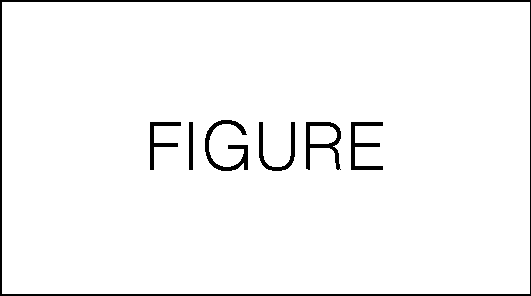
\includegraphics[width=0.8\textwidth]{DRAFT_FigsAndDocs/FIG}
	%%
	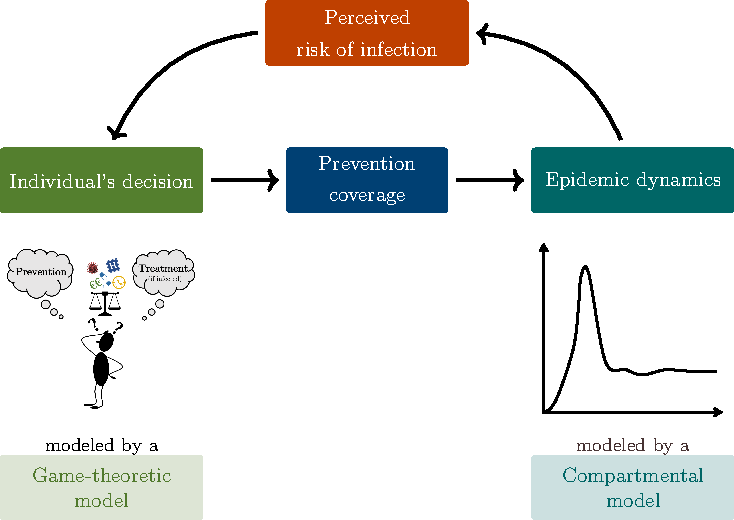
\includegraphics{Figures/Intro/TikZ_Model/ModelDiagram}
	\caption[Diagram of our hybrid model]{%
		{\bf Diagram of our hybrid model}\\
		\raggedright
		When facing an ongoing epidemic, individuals address the prevention versus treatment dilemma by evaluating the benefits and constraints of both preventive and therapeutic tools, as well as evaluating the risk of getting infected. The risk of infection perceived by individuals depends on the epidemic dynamics, which in turn depends on the efficacy and coverage of the preventive and therapeutic methods. Hence, each individual's decision may be indirectly influenced by others' decisions, since the sum of all decisions determines the voluntary prevention coverage, which impacts the course of the epidemic.
	}
	\label{ModelDiagram}
\end{figure}

\subsubsection{Modeling disease transmission at the population level}
To describe disease transmission within a population, we use a deterministic compartmental model, defined by a system of ODEs. We consider additional compartments representing individuals adopting prevention. As stated above, we do not consider that prevention is 100\% effective and thus, individuals adopting prevention can nevertheless get infected. Therefore, our model explicitly accounts for two parameters regarding prevention: coverage and effectiveness.

We use the ODE system to compute epidemiological indicators such as the incidence rate, the disease prevalence, the number of diagnoses, etc., which can be expressed explicitly as functions of the prevention parameters. By computing these epidemiological indicators at the endemic state of the system\footnote{The existence of the endemic and the disease-free equilibria is studied in detail by~\citet{Hethcote2000} for the vaccination model and by~\citet{Jacquez1988} for the PrEP model.}, we observe the behavior of the epidemic in the long run, which is used for the decision-making component of the model (see below). 

We compute the effective reproduction number from the ODE system, following the methods developed by~\citet{VanDenDriessche2002} and express it as a function of the prevention parameters (namely, the prevention coverage and effectiveness). As mentioned in~\secref{Intro:ReproductionNumbers}, we use the effective reproduction number to study the impact of the preventive methods on the epidemic. We say that the epidemic is \textit{eliminated} or \textit{averted} by the prevention method if the effective reproduction number ---a function of the prevention parameters--- is below 1. In the case where the effective reproduction decreases with prevention adoption\footnote{In the case of infectious diseases where no other preventive method is available, epidemic control induced by prevention may be characterized by the effective reproduction number being lower than the basic reproduction number.}, we say that the epidemic is mitigated or \textit{controlled} by the preventive method, since a reduction in the effective reproduction number is reflected in a reduction in the epidemic's incidence.

We first use the effective reproduction number to determine the conditions under which disease elimination or disease persistence occur, in the long run. In particular, a threshold for the prevention coverage leading to epidemic elimination can be determined. Then, the introduction of the decision-making component allows to study whether and under what conditions this theoretical threshold for epidemic elimination could be reached voluntarily. In addition, we use the effective reproduction number resulting from voluntary prevention coverage to identify a threshold for epidemic control, by finding the conditions under which individuals are motivated to adopt prevention.

\subsubsection{Modeling decision-making at the individual level}
To describe the individual's decision-making, we rely on a game-theoretical approach: a non-cooperative single-player game, where an individual is assumed to act in his own interest. 
%That is, we set a game between individuals and public health authorities, where the latter payoffs are the same as individuals' payoffs.
We assume that individuals address the prevention versus treatment dilemma by evaluating their risk of infection and by weighing the benefits and inconveniences of the preventive method versus those of treatment, which include monetary and non monetary aspects, such as price, undesired secondary effects, difficulties in access, disease morbidity, etc. In a game-theoretic framework, these factors define the perceived costs. The relative cost of prevention versus treatment thus remains a rather qualitative parameter that indicates how much more beneficial prevention is perceived over treatment.

We formally define the total expected utility as a function of the endemic risk of infection and the {\it relative cost of prevention versus treatment}, perceived by individuals. We further assume that individuals may acknowledge their true risk of infection (through official estimations of the epidemiological indicators obtained, for instance, from the transmission model, and could be communicated to the public by health authorities, healthcare providers, scientific journalists, associations, etc.), but may also make their decision based on misperception of their risk of infection (based in personal experience, rumors, peer pressure, etc.). 

\subsubsection{Model's main outcomes}
The prevention coverage that maximizes the individual's expected utility gives the probability for an individual to voluntarily adopt prevention, as a function of the model parameters. Hence, we obtain the {\it voluntary prevention coverage}, the prevention coverage reached voluntarily by the individuals who perceive themselves at risk of infection. 
%
We study the voluntary prevention coverage in terms of the preventive method's parameters: effectiveness and the relative cost of prevention versus treatment. In particular, we look for the conditions for which the voluntary prevention coverage can yield epidemic control and/or elimination, through reduction in the effective reproduction number.

